\documentclass{article}
\usepackage{amsmath}
\usepackage{amssymb}
\usepackage{enumitem}
\usepackage{algorithm}
\usepackage{listings}
\usepackage{color,xcolor}
\usepackage[T1]{fontenc}
\usepackage{fontawesome}
\usepackage{etoolbox}
\usepackage{multicol}
\usepackage{geometry}
\usepackage[colorlinks=true,linkcolor=blue,urlcolor=red,bookmarksopen=true]{hyperref}
\usepackage{tikz, pgfplots, tkz-euclide,calc}
\usepackage[outline]{contour} % halo around text
    \contourlength{1.2pt}
    \usetikzlibrary{positioning,calc}
    \usetikzlibrary{backgrounds}
    \usepgfplotslibrary{fillbetween}
    \pgfplotsset{compat=1.12} 
    \colorlet{mydarkblue}{blue!30!black}
    \usetikzlibrary{patterns,snakes,shapes.arrows,3d,patterns.meta,angles,quotes}
    \geometry{
        total = {160mm, 237mm},
        left = 25mm,
        right = 35mm,
        top = 30mm,
        bottom = 30mm,
      }
\usepackage{physics}
\usepackage{ifthen}
\usepackage[outline]{contour} % glow around text
\tikzset{>=latex} % for LaTeX arrow head
\contourlength{1.2pt}
\colorlet{myred}{red!65!black}
\tikzstyle{ground}=[preaction={fill,top color=black!10,bottom color=black!5,shading angle=20},
                    fill,pattern=north east lines,draw=none,minimum width=0.3,minimum height=0.6]
\tikzstyle{mass}=[line width=0.6,red!30!black,fill=red!40!black!10,rounded corners=1,
                  top color=red!40!black!20,bottom color=red!40!black!10,shading angle=20]
\tikzstyle{mass shadow}=[line width=0.6,rounded corners=1,loosely dashed]
\tikzstyle{rope}=[brown!70!black,line width=1.2,line cap=round] %very thick

% FORCES SWITCH
\tikzstyle{force}=[->,myred,thick,line cap=round]
\tikzstyle{Fproj}=[force,myred!40]
\newcommand{\vbF}{\vb{F}}
\newboolean{showforces}
\setboolean{showforces}{true}

\usepackage{tcolorbox}
     \tcbuselibrary{listings,skins}

\newcommand{\enter}{\raisebox{-1.8pt}{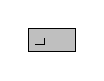
\begin{tikzpicture}[scale=0.3]
    \draw[thin,fill=lightgray] (0,0) rectangle (2,1);
    \draw (0.3,0.3) -- (0.7,0.3)--(0.7,0.6);     
\end{tikzpicture}}}

\definecolor{HIMAmuda}{HTML}{01D1FD}
\definecolor{HIMAtua}{HTML}{02016A}
\definecolor{HIMAabu}{HTML}{CBCBCC}
\definecolor{pgray}{rgb}{0.5,0.5,0.5}
\definecolor{pblue}{rgb}{0.13,0.13,1}
\definecolor{pgreen}{rgb}{0,0.5,0}
\definecolor{pred}{rgb}{0.9,0,0}
\definecolor{pgrey}{rgb}{0.46,0.45,0.48}
\definecolor{pcyan}{HTML}{D4EFFC}
\definecolor{lblue}{HTML}{00AEEF}
\definecolor{input}{HTML}{AAE1FA}
\definecolor{bg}{rgb}{0.95, 0.95, 0.92}
\definecolor{vscode}{HTML}{282A36}
\definecolor{PastelGreen}{HTML}{77DD77}

\newcommand{\inputscan}[1]{\raisebox{0pt}[1pt]{\colorbox{darkgray}{#1}}}

\usepackage{listings}

\lstdefinestyle{output}{
    language=Java,
    backgroundcolor=\color{vscode},
    basicstyle=\small\ttfamily\color{white},
    frame=none,
    escapeinside={(*}{*)},
    showspaces=false,
    showtabs=false,
    breaklines=true,
    showstringspaces=false,
    breakatwhitespace=true,
    keywordstyle=\color{white},
    }

\newtcblisting{RunCode}[1][enhanced,drop shadow]{
    arc=0pt, outer arc=0pt,
    boxsep=1pt,
    boxrule=2pt,
    auto outer arc,
    colback=vscode,
    colframe=bg,
    listing only, 
    listing style=output,
    title=\color{black}Ex. Output,
    #1
    }
\newtcblisting{RunCodeMore}[1][enhanced,drop shadow]{
    arc=0pt, outer arc=0pt,
    boxsep=1pt,
    boxrule=2pt,
    auto outer arc,
    colback=vscode,
    colframe=bg,
    listing only, 
    listing style=output,
    #1
    }

\newtcolorbox{hint}[1][]{
    colback=PastelGreen!5!white, 
    colframe=PastelGreen!75!black,
    fonttitle=\bfseries, 
    colbacktitle=PastelGreen!85!black,
    enhanced, 
    attach boxed title to top left={yshift=-2mm}, 
    title=Hint,
    before upper=\renewcommand\thempfootnote{\Roman{mpfootnote}},
    #1
}

\newtcolorbox{example}[1][]{
    colback=pgreen!5!white, 
    colframe=pgreen!75!black,
    fonttitle=\bfseries, 
    colbacktitle=pgreen!85!black,
    enhanced, 
    attach boxed title to top left={yshift=-2mm}, 
    title=Example,
    before upper=\renewcommand\thempfootnote{\Roman{mpfootnote}},
    #1
}

\newtcolorbox{req}[1][]{
    colback=lblue!5!white, 
    colframe=lblue!75!black,
    fonttitle=\bfseries, 
    colbacktitle=lblue!85!black,
    enhanced, 
    attach boxed title to top left={yshift=-2mm}, 
    title=Input,
    before upper=\renewcommand\thempfootnote{\Roman{mpfootnote}},
    #1
}

\newtcolorbox{out}[1][]{
    colback=HIMAtua!5!white, 
    colframe=HIMAtua!75!black,
    fonttitle=\bfseries, 
    colbacktitle=HIMAtua!85!black,
    enhanced, 
    attach boxed title to top left={yshift=-2mm}, 
    title=Output,
    before upper=\renewcommand\thempfootnote{\Roman{mpfootnote}},
    #1
}

\renewcommand{\thesubsection}{\arabic{subsection}}
\newcommand{\R}{\mathbb{R}}
\newcommand{\Z}{\mathbb{Z}}
\newcommand{\N}{\mathbb{N}}
\renewcommand{\figurename}{Gambar}

%\setminted[java]{bgcolor=bg,fontsize=\small,frame=single,bgcolorpadding=1mm,escapeinside=||}

\title{\textbf{Week 3 Assigment}}
\date{11 Maret 2025}
\author{Teosofi H.A \& Hafidz M.}

\begin{document}
  \maketitle
  \pagenumbering{gobble}
  \section*{Tugas Mandiri}
  \begin{enumerate}
    \item Buatlah kode program dengan menggunakan algoritma \textit{binary search} untuk mendapatkan nilai pembulatan dari akar bilangan bulat.
    \begin{req}
        $1 \leq n \leq 10^9$
    \end{req}
    \begin{out}
        $\lfloor\sqrt{n}\rfloor$ 
    \end{out}
    \begin{RunCode}
sqrt(0) = 0
sqrt(1) = 1
sqrt(2) = 1
sqrt(3) = 1
sqrt(4) = 2
sqrt(5) = 2
sqrt(6) = 2
sqrt(7) = 2
sqrt(8) = 2
sqrt(9) = 3
sqrt(10) = 3
...
    \end{RunCode}
    
    \item Diberikan sebuah matriks $A$ berukuran $n \times m$ yang berisi bilangan bulat non-negatif. Kemudian terdapat matriks $A'$ dengan ketentuan sebagai berikut:
    \begin{itemize}
      \item Ukuran matriks $A'$ sama dengan ukuran matriks $A$.
      \item Kolom ke-$i$ pada $A'$ berisi elemen-elemen pada kolom ke-$i$ matriks $A$ yang sudah diurutkan dari yang terkecil ke yang terbesar (atas yang paling kecil). 
    \end{itemize}
    Buatlah program dengan input sebuah matriks $A$ dan mengeluarkan output berupa matriks $A'$.
    \begin{req}
        \begin{itemize}
            \item $1 \leq n \leq 100$
            \item $1 \leq m \leq 100$
            \item  $0 \leq a_{ij} \leq 10^9$
        \end{itemize}
    \end{req}
    \begin{out}
        $A'\in \R^{n \times m}$
    \end{out}
    \begin{example}
        Contoh matriks $A$ dan $A'$ yang memenuhi:
        \begin{align*}
            A_1 &= \begin{bmatrix}
                1 & 2 & 7 \\
                0 & 5 & 6 
            \end{bmatrix} &\quad
            A_1' &= \begin{bmatrix}
                0 & 2 & 6 \\
                1 & 5 & 7
            \end{bmatrix}
        \end{align*}
        \begin{align*}
            A_2 &= \begin{bmatrix}
                1 & 21 \\
                0 & 5 
                17& 8\\
                7 & 29\\
            \end{bmatrix} &\quad
            A_3' &= \begin{bmatrix}
                0 & 5 \\
                1 & 8 \\
                7 & 21 \\
                17 & 29 
            \end{bmatrix}
        \end{align*}
        \begin{align*}
            A_3 &= \begin{bmatrix}
                12 & 20 & 7 & 40 & 13 \\
                0 & 5 & 6 & 1 & 2 \\
                0 & 43 & 0 & 53 & 78 \\
                1 & 13 & 90 & 0 & 65 \\
                0 & 0 & 1 & 0 & 0 
            \end{bmatrix} &\quad
            A_3' &= \begin{bmatrix}
                0 & 0 & 0 & 0 & 0 \\
                0 & 5 & 1 & 0 & 2 \\
                0 & 13 & 6 & 1 & 13\\
                1 & 20 & 7 & 40 & 65 \\
                12 & 43 & 90 & 53 & 78
            \end{bmatrix}
        \end{align*}
    \end{example}
  \end{enumerate}
\end{document}